% Chapter Template

\chapter{Implementation} % Main chapter title

\label{Chapter3} % Change X to a consecutive number; for referencing this chapter elsewhere, use \ref{ChapterX}

\section{Introduction}
In the previous chapters, we discussed about the context of the work and the technologies, both software and hardware required to execute the project. In this chapter, we would go through methods and steps 
with which we can utilise those technologies to produce results. In our implementation, we wish to study the behavior of robot with respect to it's neighbourhood obstacles. To achieve studying of goals, we will use the relative position of the robot
with respect to the obsatcles and result in a log file for data mining purposes.

\section{Environment Development}
The simulation environment used in the project is Gazebo11 \cite{1389727}. Gazebo is a simulation environment where we can create a Digital Twin \cite{8901113}. ROS framework utilizes Gazebo as 
the simulation environment for both our robot as well as the obsatcle environment. To simply simulate the robot into Gazebo, we need to define \textit{launch} files, which contain arguments to define the robot and it's specifications.
In a launch file, we define the initial position of the robot, the world file we might use, import the neccesary equipments of the robots and define the sensors of the robot, it's base, and the manufacturer of each.
The equipments are defined by using \textit{xacro} files which are saved in the same directory. We can also call other processes and scripts to run, as well as visualization in the launch file. The \textit{launch} file also helps us define and call \textbf{AMCL} launch file,
which helps us localize the robot in the environment frame. The launch files contain arguments to visualize the processes with RViz (ROS Visualization Tool). The launch file is programmed in XML-like structure.
In the project, we have floor tiles, square boxes and walls surrounding the environment. These entities can be created in CAD and imported as we intend to implement. These entities are stored in \textit{.gazebo} directory 
and therefore can be used to develop other environments with different configurations. The digital twin developed along with the robot is noted and studied from the top at \textit{god's eye view}.
In ROS package, launch folders contain the launch files, which call models from models and world directory. Note that, models are building blocks of world files. World files with different configurations are stored in \textit{worlds} directory in the ROS package.

\begin{figure}[th]
    \centering
    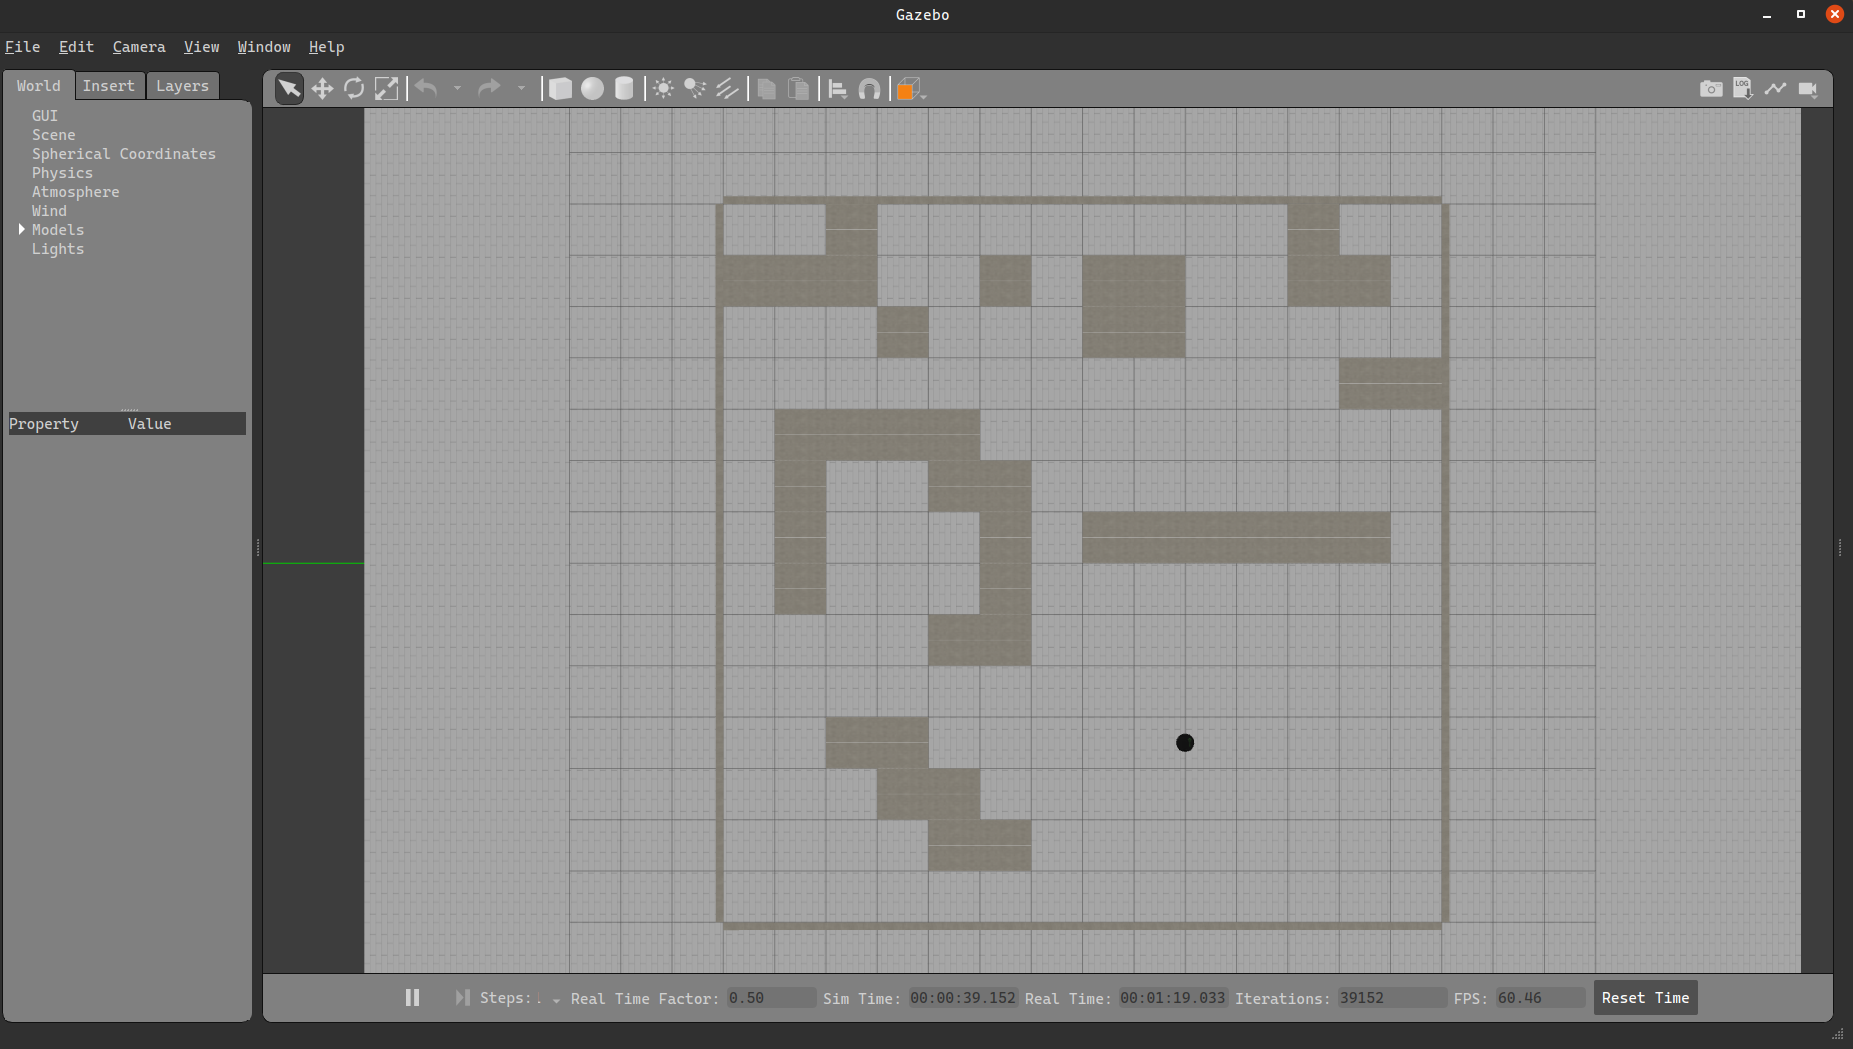
\includegraphics[width=\textwidth]{Figures/base_god_eye_world.png}
    \decoRule
    \caption[]{God's eye view of 14x14 grid}
    \label{fig:14x14grid}
\end{figure}

\begin{figure}[th]
    \centering
    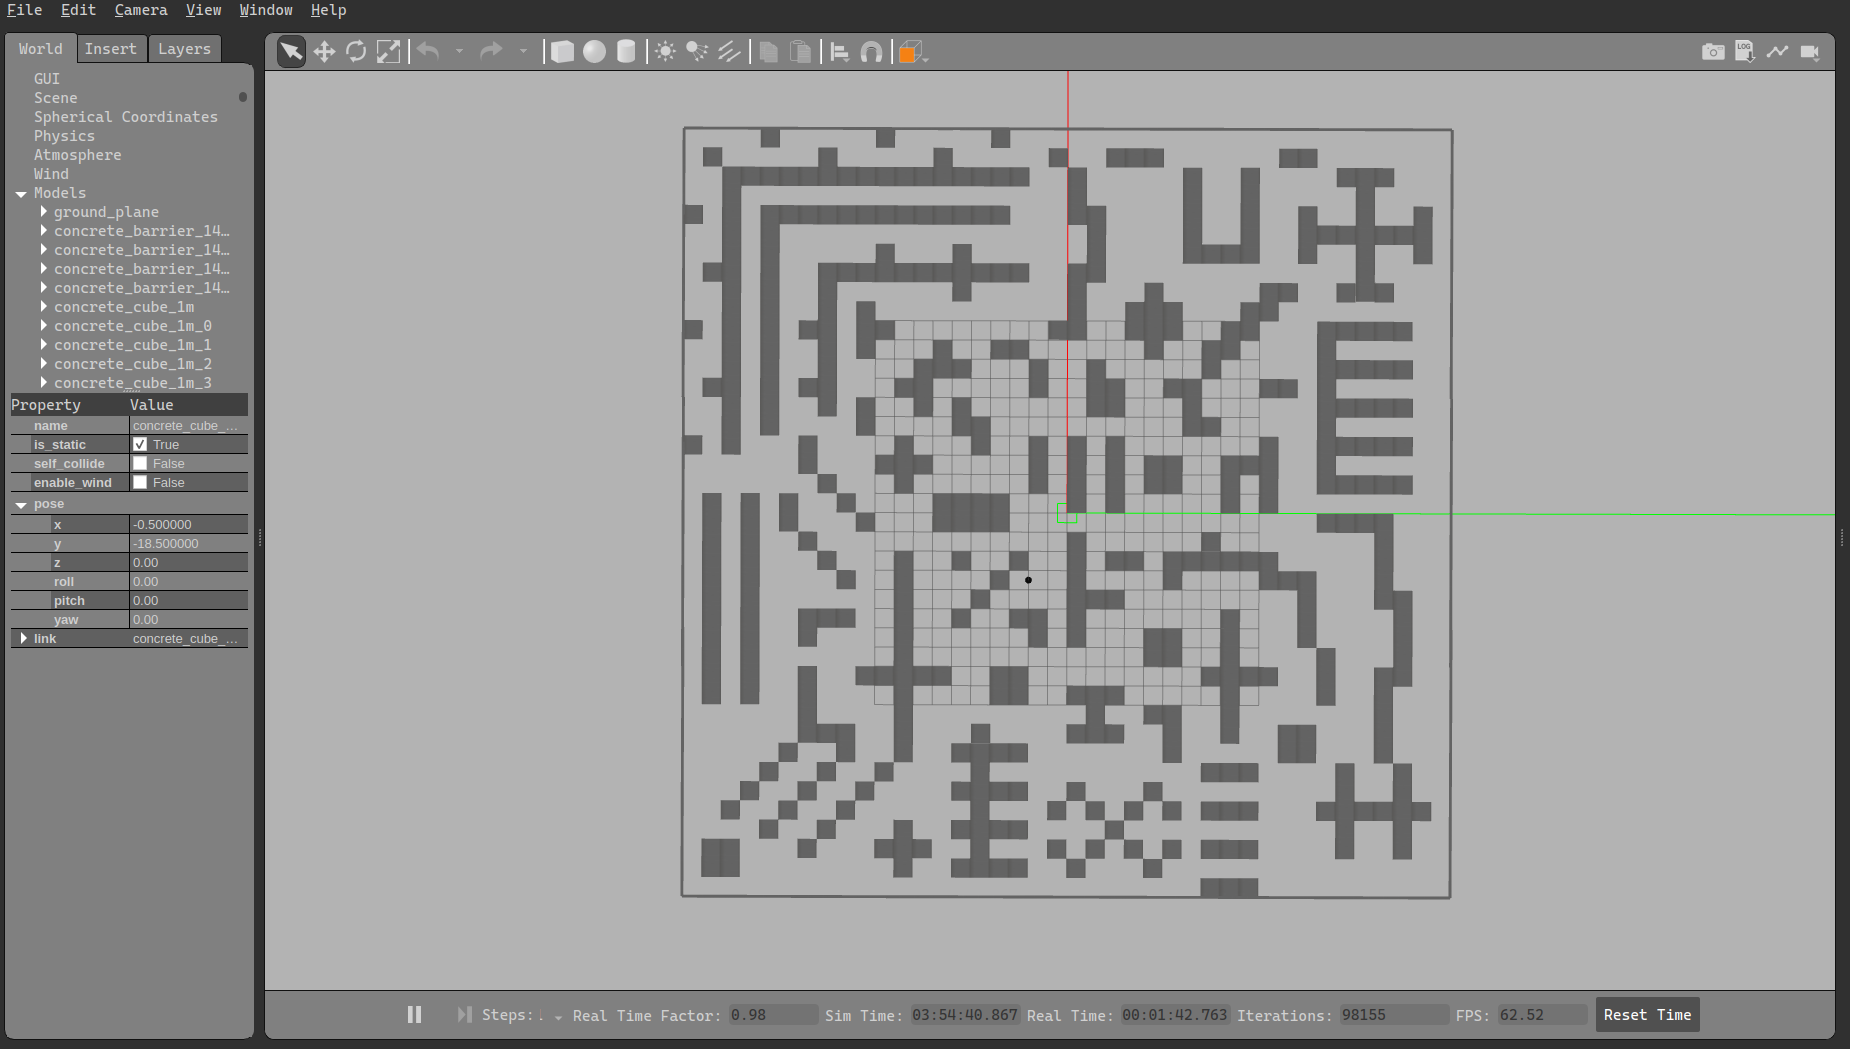
\includegraphics[width=\textwidth]{Figures/30_30_god_eye_world.png}
    \decoRule
    \caption[]{God's eye view of 30x30 grid}
    \label{fig:30x30grid}
\end{figure}

\section{SLAM}
SLAM (Simultaneous Localization and Mapping) is done by simulating the turtlebot in a particular environment. 
As the robot does not know anything about the environment, a \textit{teleoperation} command, i.e using the keyboard
to move the robot around the environment. As the robot has a 360\textsuperscript{o} LIDAR sensor, concurrent mapping 
and localization is done. The map is generated and saved for further global path planning and navigation.The user, controlling the 
robot stop the teleoperation will stop moving around the robot when the mapping is done completely.
In SLAM methods in ROS, we can use different methods to execute SLAM such as "gmappping" (\url{wiki.ros.org/gmapping}) which uses a two
dimensional occupancy grid map describing the configuration space. Another such method is "cartographer" (\url{wiki.ros.org/cartographer})
utilizing an algorithm employing loop closure method. In our work, we implemented the \textit{gmapping} package to implement SLAM.

\begin{itemize}
    \item Simulate the robot in environment with \textit{launch} files.
    \item Using turtlebot package to initiate SLAM.
    \item Starting the teleoperation node in another terminal.
    \item Moving the robot around the environment to record the map.
    \item Saving the map.
\end{itemize}

\begin{figure}[th]
    \centering
    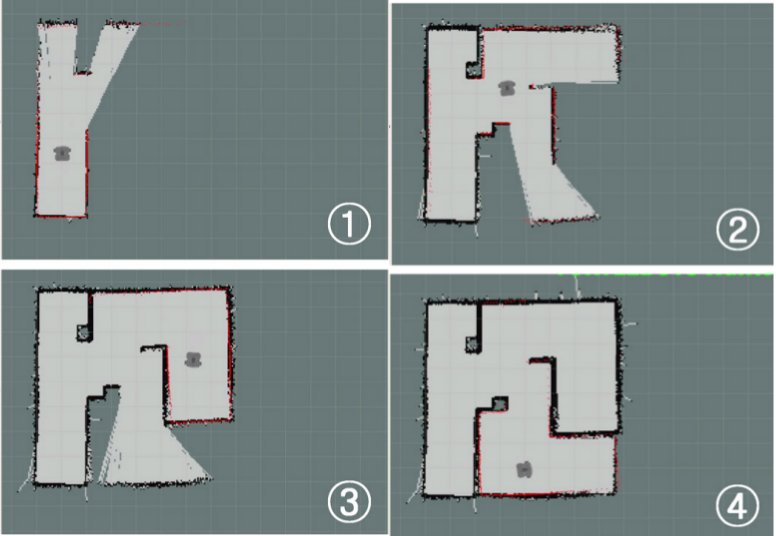
\includegraphics[width=\textwidth]{Figures/SLAM.png}
    \decoRule
    \caption[]{Step-by-Step SLAM}
    \label{fig:Step-by-StepSLAM}
\end{figure}

\section{Navigation}
Navigation in ROS based environment is done through the navigation stack. Navigation stack is an open-source framework in ROS which accompanies everthing 
required for a robot to move from a point to the other. The navigation stack is completely configurable, and developer can add 
their code into the stack when we wish to. Navigation stack is available on Github, for anyone to use and utilise. 
ROS Navigation stack is on a conceptual level. The information is taken from odometry, and goal pose of the robot and sensors. 
Navigation stack deals with publishing velocity to the robot controller, the values will be published
according to the need to reach the goal pose. There are many prerequisites in Navigation Stack, 
\begin{itemize}
    \item The robot should be running ROS.
    \item coordinate frame of the robot, i.e \textit{tf transforms} should be known.
    \item global plan coordinate frame of the robot should be known.
    \item correct \textit{message} files to exchange information in between processes.
\end{itemize}
To fully setup the essential navigation stack, it's configuration can be done through \url{http://wiki.ros.org/navigation}
In our implementation, we are using the local path planner but we are not employing the LIDAR sensor to avoid obstacle dynamically.
The robot in our implementation, does not intend to path plan in a dynamic fashion. Instead, we wish to read the behaviour of the robot in relation with it's global path plan.
In the data flow in Navigation Stack, odometry and LIDAR are the chosen combination. Odometry is the most important information in the control.
As we wish to \textit{see and record} the behavior of the robot from a god's eye view, we will only use Odometry information to
see the \textit{x and y} values of the robot in relation to the coordinate frame. The goal pose is chosen from using the ROS Visualization tool.
Navigation stack will be turned on to work, when a goal pose is chosen. The navigation then publishes the trajectory poses and velocity from the 
robot's controller. The transform tree, is utilized to specify the motion constraints of the robot like it's height and width of the mobile base.
There are various such parameters attached in the \textit{config} folder describing different patterns in numerous \textit{.yaml} files.

\subsection{Customized Global Planner Algorithm}
In our implementation, the robot's possible movements are only in 4 directions. We don not wish the optimization of the path, instead we wish to focus
on defining the movement in those directions. Thus, after defining the \textit{global costmap} and it's grids. The algorithms should only iterate and explore
over the \textit{top, left, right and down} nodes only at each and every step.
In the figure 3.4, the node \textbf{R} is an obstacle, which is describe as a value greater than 1 in global costmap configuration.
Thus, the robot's global planner can not explore that node and further nodes that can exist and explored from using \textbf{R} as a referemce point.
As the nodes \textbf{L,P and V} are free, in the next step the robot's global planner will proceed to explore the other nodes built upon those.
\begin{figure}[th]
    \centering
    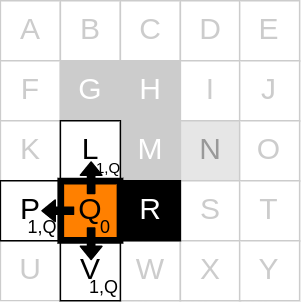
\includegraphics[width=0.4\textwidth]{Figures/grid_map_expansion_02.png}
    \decoRule
    \caption[]{Exploration Strategy of Nodes}
    \label{fig:NodeExploration4Node}
\end{figure}
Let's consider that \textbf{L} was node chosen in order to move to the goal pose. We will proceed to explore the nodes adjecent to the \textbf{L} node.
In figure 3.5, the node \text{L} has 4 neighbours, namely \textbf{K,G,M,Q}. As \textbf{G and M} are obstacles with \textbf{Q} being the previous explored node.
We have no other option to chose node K as our next node.

\subsubsection{Strategies of Planning}
As we discussed that, there are three algorithms implemented in our project which are namely, \textit{Dijkstra's Algorithm, A\textsuperscript{*} Algorithm and GBFS algorithm}.
These three algorithms will follow a similar node exploration strategy but the incentives to explore a new node will differ from algorithm to algorithm, resulting in different strategies to reach the goal pose node.

\begin{figure}[th]
    \centering
    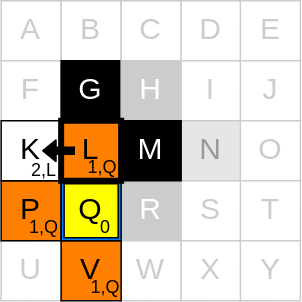
\includegraphics[width=0.4\textwidth]{Figures/grid_map_expansion_03.png}
    \decoRule
    \caption[]{Next stage of exploration.}
    \label{fig:NextNodeExploration4Node}
\end{figure}






